\documentclass[conference]{IEEEtran}

\ifCLASSINFOpdf

\else

\fi


\usepackage{graphicx}

% correct bad hyphenation here
\hyphenation{op-tical net-works semi-conduc-tor}


\begin{document}

\title{The Creation of Co-evolution \\ by the Hands of God}



\author{\IEEEauthorblockN{Enrico Rotundo, Selene Beaz Santamaria, Andrea Borchelli Peperoni, Tommie Limberjack}
\IEEEauthorblockA{Vrije Universiteit Amsterdam \\
Amsterdam, Netherlands\\
Email: Enrico@smellLikePizza.italia}}



\maketitle


\begin{abstract}
In the robotics context, intelligent behaviours are often achieved using neural networks as controllers evolved with an evolutionary algorithm.
In the case of multiple individuals within a species, controllers can be either homogeneous or heterogeneous.
In this paper, we use the competitive co-evolution in order to investigate its interaction with the relation between the homo and hetero cases.
% TODO: add what we have discovered
\end{abstract}


\IEEEpeerreviewmaketitle


\section{Introduction}
Evolutionary algorithms (EA) are biological inspired algorithms that evolves over time through generations of individuals. 
The evolution is usually controlled such that next generations improve along the runs.
In the robotics field, evolutionary algorithms can be used to evolve the  behaviour controller of an individual.
Neural Networks (NN) are functions estimators or approximators nautal inspired by animals nervous systems, their design allows them to accepts high dimensionaity inputs.   
Properly trained Neural Networks can be used to control the behaviour of a robot, where inputs are sensors based observations and weights are evolved by an evolutionary algorithm.
A whole evolution process can be run as a virtual simulation which exploits the current computer's computational power in order to evaluate many generations in a reasonable time.
Robotics uses both NN and EA in order to evolve intelligent behaviours that can pursue some goals.
Tasks composition and complexity can vary based on the specific use case, in general it is object of many research investigations which aim to solve different tasks.
For instance, tasks can be relatively small (e.g., moving objects) or more based on collaboration between a number of individual.
Research investigations analyse collective behaviour in order to asses to which extent collaboration between individuals is feasible.  

In this paper, we consider competitive co-evolution within a herding task which consists in a number of shepherds that herd a sheep into a corral.
Here we focus on evolving NNs as controllers for the agents.
Controllers can be assigned to agents with different approaches, the homogeneous consists in using the same controller for each individual of a specie (e.g., shepherds) while the heterogeneous assigns a different NN for each agent.
Moreover, the task complexity can be increased by varying or introducing new agents like adding a fox.

We recap our objectives in the following list:

\begin{itemize}
	\item To compare homogeneity versus heterogeneity.
	\item To estimate the effect of increasing the task difficulty.
 	\item To develop controlled experiments through software simulations, using ad hoc Java libraries.
	\item To collect comprehensive results data.
\end{itemize}
 
\subsection{Research questions}
In the herding task, shepherds and sheep have opponents behaviours in the sense that their goals are opposite.
While the shepherds try to herd sheep into the corral, the sheep tries to run away from the left side of the pasture.
Thus, competing species can be co-evolved fighting against each others.
Furthermore, the task complexity can be influenced by varying different parameters such as the number of sheep or their speed.

The following research questions assume intelligent sheep within a herding task:
 
\begin{enumerate}
	\item How does the competitive co-evolution affect the relation between homogeneous and heterogeneous (dog’s) controllers in a co-evolutive herding task?
	\item How does increasing the difficulty (e.g.: by increasing the sheep’s speed) of a single task increase the necessity for heterogeneous controllers?
	\item How does increasing task complexity by adding more sheep affects the effectiveness of herding?
\end{enumerate}

\subsection{Hypothesis}
\label{sec:hypothesis}
The following hypothesis are in one to one relationship with the aforementioned research questions:

\begin{enumerate}
	\item Shepherds’ fitness in the heterogeneous case is overall higher than in the homogeneous case.
	\item Shepherds’ fitness in the heterogeneous case and sheep’s speed are inversely related, such that fitness decreases as speed increases.
	\item Shepherds’ fitness in the heterogeneous case and sheep’s multiplicity are inversely related, such that fitness decreases as speed increases.
\end{enumerate}

We now consider $H_1$, we leave the testing of the others as future work. The $H_0$, namely null hypothesis, is ``Shepherds’ fitness in the heterogeneous case is equivalent to the one of the homogeneous''.

\section{Literature}
 
\subsection{Coevolution}
It was as early as 1964 when Ehrlich and Raven focused their paper \cite{ehrlich1964butterflies} describing the effects of coevoultion in butterflies and plants.

In 1980 Janzen's \cite{janzen1980coevolution} formalised a clear definition for coevolution:
`` 'Coevolution' may be usefully defined as an evolutionary change in a trait of the individuals in one population in response to a trait of the individuals of a second population, followed by an evolutionary response by the second populations to the change in the first.''


\subsection{Competitive Coevolution}
Dawkins and Krebs described in their 1979 paper: ``Arms Races between and within Species'' \cite{dawkins1979arms}, the dynamics of, and created terminology for, competitive coevolution. Provided are examples of manifestations of competitive coevolution in natural systems.

In \cite{stanley2004competitive} Stanley and Miikkulainen showed that through the complexification of agent controllers in a competitive co-evolutionary setting, the controller's added complexity can be utilized through the generation of more advanced strategies as complexity increases.


\subsection{Homogeneity vs Heteroheneity in ANN's}
\cite{potter2001heterogeneity} performed a study to a tradeoff of homogeneity versus heterogeneity in the control systems of robots by allowing teams to coevolve their high-level controllers given different levels of difficulty of the task
Hypothesised was that: ``\textit{simply increasing the difficulty of a task is not enough to induce a team of robots to create specialists.}''
Task difficulty was varied by replacing one adversary's passive controller with an active variant supposedly proving that increased difficulty did not justify the use of heterogeneous controllers.
However, increased difficulty was never implemented structurally nor tested methodologically. 



\section{Model}
TODO

\subsection{NN design}
TODO

\subsection{Evolution of NN controllers}
TODO

\subsection{Shepherds controllers}
TODO

\subsection{Sheep controllers}
TODO

\section{Implementation}
TODO

\section{Experiment}
\label{sec:experiment)
In this section we detail the design of the experiments performed in this paper.
For the sake of shortness, we go just show the experiment that considers the $H_1$ listed in ~\ref{sec:hypothesis}.
This experiment involves the following entities:

\begin{itemize}
	\item 2 homogeneous shepherd’s vs 1 (intelligent) sheep
	\item 2 heterogeneous shepherd’s vs 1 (intelligent) sheep
\end{itemize}


\section{Results}
In this section we present the results of the experiment detailed in Section ~\ref{sec:experiment}.

\begin{figure}[ht]
\centering
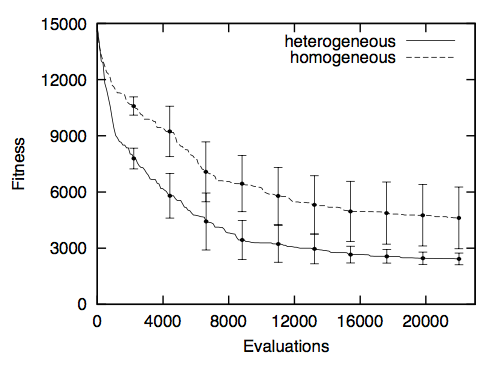
\includegraphics[width=3.3in]{imgs/homo_vs_hetero.png}
\caption{TODO.}
\label{fig:homo_vs_hetero}
\end{figure}

\section{Conclusion}
The conclusion goes here.

\subsection{Future work}
TODO

-In a competitive co-evolution, how does increasing task complexity by adding more sheep affects the effectiveness of herding? %TODO: fix

-[In a competitive co-evolution, do heterogeneous sheep perform better than homogeneous?] %TODO: fix



\bibliographystyle{abbrv}
\bibliography{bibliography}



\end{document}

